%
\documentclass[Proceedings]{ascelike}
\usepackage[utf8]{inputenc}
% Some useful packages...
%
\usepackage{graphicx}
\usepackage{subfigure}
\usepackage{amsmath}
\usepackage{amsfonts}
\usepackage{amssymb}
\usepackage{amsbsy}
\usepackage{times}
\usepackage{float}
\usepackage{algorithm}
\usepackage{algpseudocode}


% Definitions
\DeclareMathOperator*{\argmin}{arg\,min}

%
%
% Place hyperlinks within the pdf file (works only with pdflatex, not latex)
% \usepackage[colorlinks=true,citecolor=red,linkcolor=black]{hyperref}
%
%
% NOTE: Don't include the \NameTag{<your name>} if you have selected
%       the NoPageNumbers option: this leads to an inconsistency and
%       a warning, and the NameTag is ignored.
\NameTag{Perryman R., Nassif L., Mobayed A.}
%
%
\begin{document}
%
% You will need to make the title all-caps
\title{ANALYZING TRANSPORTATION SERVICES WITH CENTRALIZED ROUTING}
%
\author{
Richard Perryman
\thanks{Student ID: 1003874925},
Loic Nassif
\thanks{Student ID: 1001309808},
Amjad Mobayed
\thanks{Student ID: 999819987}
}
%
\maketitle
%
\begin{abstract}
The popular approach to match customers and vehicles in a taxi-like service (e.g. Uber) is to assign the closest available cab to the newly appeared customer. Once assigned, the cab's destination is locked to the customer's location. We decide to look into the idea of recalculating the optimal assignment of cabs and customers in a city map where customers appear following a random distribution. We investigate the efficiency of changing the routes of already assigned cabs to different customers to minimize the overall average waiting time of customers. We apply our model to two different situations; one where the cabs are human-driven and the other when the cabs are self-driven. We found that for all cases, rerouting or not, human driven or self-driven, the results are very similar. By small margins, the most efficient method was to have self-driving cabs in a rerouting model.
\end{abstract}
%
% Some keywords, using a new command: \KeyWords{}
%
\KeyWords{Vehicle Routing Problem, Centralized Routing, Probabilistic Model, Heuristic Algorithms}
%

\newpage

\section*{Introduction}

\subsection*{Background}

The problem we are tackling falls under a larger set of problems named Vehicle Routing Problems (VRP). These problems have been studied very extensively in the past 60 years\cite{VRP}\cite{SA}, and the heuristic methods developed and analyzed in past research will influence our choices of algorithms. The VRP is the challenge of finding optimal paths for one or more vehicles to one or more customers scattered around a location such as a city. This can be solved with a number of different approaches. These approaches can usually be classified as exact algorithms or heuristic, or approximate, algorithms. The problem with exact algorithms, such as direct search trees, is that the VRP is an NP-hard problem. This makes solving the problem for a realistic number of vehicles and customers impossible. Exact algorithms can solve the problem for a couple dozen customers\cite{Exact}. This is simply not useful for our purposes and so we turn to heuristic approaches. The VRP can often times be represented as a programming problem and as such can be solved using relaxation methods such as Lagrangian relaxation, where the Lagrangian multipliers are used as a weighted penalty for violating the inequality constraints, instead of making these constraints completely binding. A popular search algorithm that we will use a variation of in our model is called the $A^*$ search algorithm. The basic idea of $A^*$ is that the algorithms will consider all possible, reasonable, combinations of nodes between the vehicle and the customer and pick the one that minimizes a particular cost, in our case the distance travelled by the vehicle to the customer. \\

It seems that none of the previous literature looks at the VRP when there is a time-dependent aspect to the system. As more customers appear randomly throughout the city, the optimal path between vehicles and customers may change in such a way that reassigning vehicles-customers pairings may reduce the overall travel and wait time.

\subsection*{Motivation}

There are a few reasons why we might suspect this to be a good idea to investigate. In terms of practicality, reducing customer wait time increases customer satisfaction, while reducing travel time reduces maintenance cost for the business, and increases the ability to serve more customers with fewer vehicles. The idea of rerouting may seem to be a very real possibility for the near-future of self-driving cabs, since machines can react instantaneously to immediate and multiple rerouting changes that a human driver may not be able to handle as efficiently.

\subsection*{The Model}

A large part of the development of our model is the construction of our model city from which all of our tests are gathered from. The way that a city is modeled is to represent each intersection as a node in a graph. The challenge then is to find a way to link up thousands of nodes to form a city network. It is in our effort to create the network where most of our model assumptions arise. To begin with, we assume each link, which is analogous to an edge on a graph, is connected in a straight path. This is not a bad assumption to make for a large metropolitan city, since most of these cities are arranged in a grid-like configurations and most of their major roads are straight. The distance from one node to its neighbouring node is a value saved within the node. The next assumption is tied to the data that is available to us online. We tie the frequency of customers appearing at a given intersection to the density of pedestrians at the intersection. This naturally means that for an intersection to be useful to us in this model, we need to find data on the pedestrian density for each intersection. The Toronto Open Data Catalogue has a data set of vehicle and pedestrian volumes over the 8-hour traffic peak time at intersections that have traffic signals\cite{TorontoTraffic}. This eliminates a lot of Toronto's intersections. Another Toronto data set, one simply registering all intersections within the City of Toronto\cite{TorontoIntersections}, has a count of about 50000 intersections. Contrasting that to $\sim2000$ intersections with volume data shows that a majority of Toronto cannot be accurately modeled. \\

We continue our assumptions with the reasonable thought that every node can be accessed, through some path, from any other node. This is usually true for most cities, although we do not consider things such as one-way streets or closed-off streets that may inhibit the path of the vehicle. \\

Another important aspect of our model is how customers and vehicles behave. We model the customer appearance rate at an intersection using a random process. The likelihood of customers appearing is scaled by the volume of pedestrians at the given intersection. This is using the assumption that more busy intersections will harbor more customers. If we consider human drivers, then we introduce a reaction delay time. In many cases, the rerouting may occur unexpectedly and the human driver may need a few seconds to react to the change. When using self-driving cars, this constraint is not considered. \\

The centralized system that assigns the employees driving vehicles to the waiting customers is modeled simply as a
computer that has access to the location of each customer and each vehicle. This computer calculates routes for the
employees to follow along with how far the vehicle would have to travel using an extension of Dijkstra's Algorithm~\cite{Dijkstra1959}
commonly called \( A^{*} \), which uses the location of the intersections on the Earth to improve performance.
The computer then uses these routes to find a close to optimal set of pairings in order to minimize the distance
traveled by the vehicles. The results are not exact due to some pruning done to meet time constraints, but there is
very rarely a significant difference.

\section*{City Modeling}

There are no real benefits for our goals to model Toronto accurately. Our objective is to be able to model an example city accurately. We would simply need a graph that accurately describes the general patterns of a metropolitan city, and so a crude approximation of Toronto suffices. There are a few ways of linking the nodes. The first one is to simply link them randomly. The danger with doing so is that clustering may occur. That is, sub-networks of nodes, detached from all other nodes, may start to form. To prevent this, before randomizing the links, We connect all nodes in a successive chain, ensuring that all nodes are connected. \\

Odd patterns that do not capture the structure of a city may form if we create a network randomly. A better approach would be to connect nodes that are geographically near-by. We can allow a node to connect to its four closest nodes and do so for all other nodes in the graph. Complexity can be added to this model of joining nodes. For example, some intersections could be linked to intersections that are much further away from its four nearest neighbours, such as pseudo-highway like street connections. The data retrieved from the City of Toronto saves the locations of the intersections in a MTM 3 Degree Zone 10 NAD27, WGS84 Latitude/Longitude projection. That is the latitude and longitude are in degrees. We first convert these coordinates in radian and apply the Haversine formula to find the distance, since we are dealing with two points on a curved surface,
\begin{equation}
    d = 2r\arcsin\Bigg(\sqrt{\sin^2\bigg(\frac{\varphi_2 - \varphi_1}{2}\bigg) + \cos\varphi_1 \cos\varphi_2 \sin^2\bigg(\frac{\lambda_2 - \lambda_1}{2}\bigg)}\Bigg)
\end{equation}

where $r$ is the radius of the earth, $\varphi_2$ and $\varphi_1$ are the latitudes of point 2 and point 1, respectively, and $\lambda_1$ and $\lambda_2$ are the longitude of point 1 and point 2, respectively.

\begin{figure}[H]
    \centering
    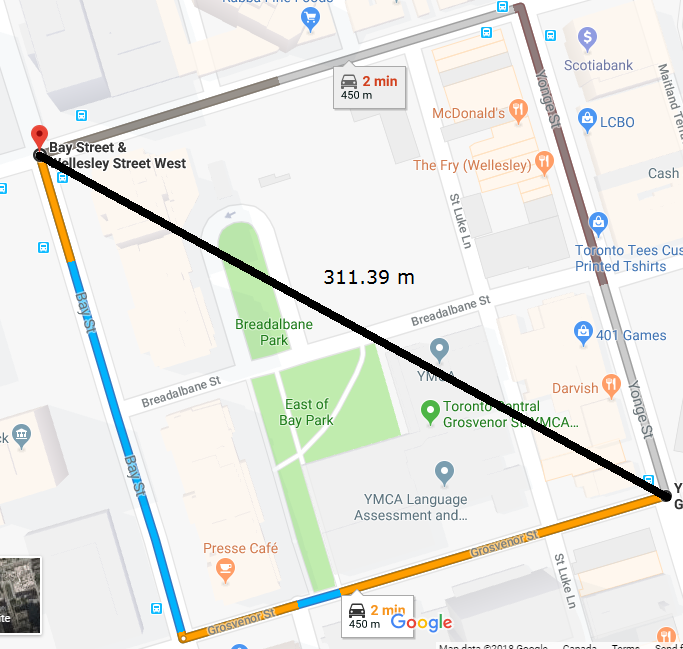
\includegraphics[scale = 0.55]{shortcomings.png}
    \caption{An issue highlighted by the fact that not all intersections are considered in our model.}
    \label{fig1:short}
\end{figure}

Shortcomings to this approach exist. For example, in Figure \ref{fig1:short}, the black line drawn is how our link of the two nodes is constructed. This is of course not what the real map looks like, and so accuracy in simulating Toronto is diminished. On the other hand, the actually geometry of the graph is not as important as is its link density connection. The average intersection in our model is linked to 4.0 other intersections. This is similar to what a city like Toronto would be expected to have. \\

The area of Toronto that we consider is from the latitude 43.591686475 to latitude 43.85545 and longitude -79.63929 to longitude -79.3896419. This is equivalent to the bottom left corner being at 97 City Centre Dr, Mississauga, ON L5B 1M7, Canada and the top right corner at 35 West Beaver Creek Rd, Richmond Hill, ON L4B 1K4, Canada. Figure \ref{fig1:range} demonstrates such a range. The number of intersections in that range is about 26862. We captured about 1210 of these intersections. This might seem little, but do note that all intersections that have vehicle and pedestrian volume data are intersections with traffic signals, and these intersections are the ones that tend to be larger, and more important for our purposes, than the intersections without traffic signals.

\begin{figure}[H]
    \centering
    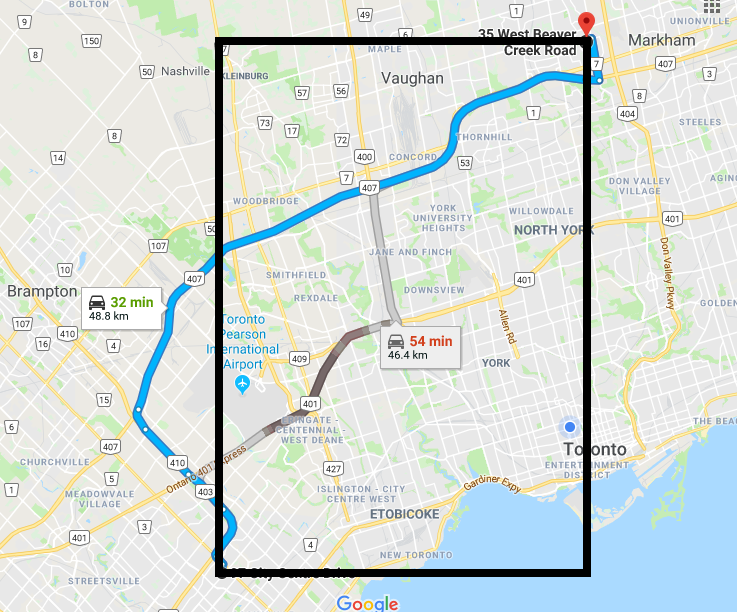
\includegraphics[scale = 0.55]{range.png}
    \caption{The extent of our model covering parts of Toronto.}
    \label{fig1:range}
\end{figure}

\begin{figure}[H]
    \centering
    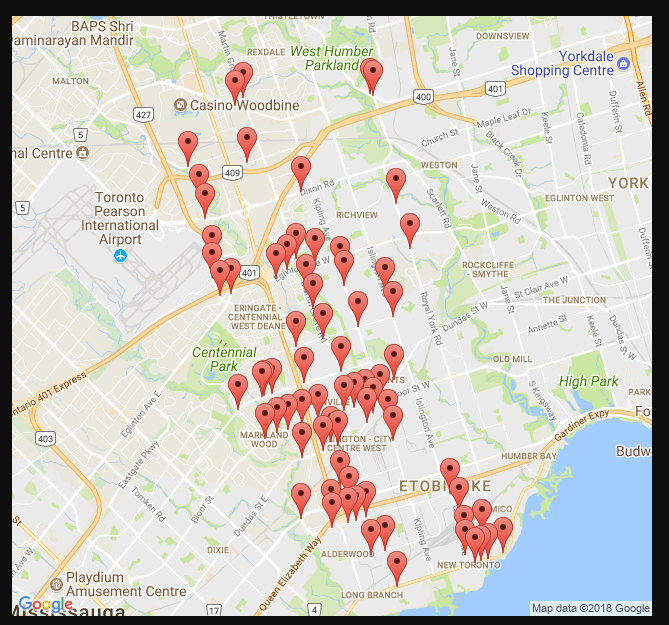
\includegraphics[scale = 0.55]{sample.png}
    \caption{A small representation of our intersections distribution in a small area of our model's region.}
    \label{fig1:sample}
\end{figure}

Table \ref{tab1:toronto} shows the contrast between our model's and Toronto's distribution of intersection types. The meaning of each specific type is not very relevant to discuss, but the point is that our model samples a large portion of Minor-Single Level intersections, which is the dominant type of intersection in Toronto. What our model fails to capture are Lesser-Single Level intersections, which our model has none of, but consists of a large portion of Toronto's infrastructure. This is explained by the fact that Lesser-Single Level intersections are intersections that involve one-way roads. One-way roads are usually associated with smaller street intersections which normally do not posses traffic signals, which is a binding criteria for our model.

\begin{table}[H]
\centering
\caption{Distribution of street types between our model and Toronto in the area considered.}
\label{tab1:toronto}
\begin{tabular}{|c|c|c|}
\hline
                                                                                       & \begin{tabular}[c]{@{}c@{}}Our Model\\ (1210)\end{tabular} & \begin{tabular}[c]{@{}c@{}}Toronto\\ (26862)\end{tabular} \\ \hline
\begin{tabular}[c]{@{}c@{}}Minor-Single\\ Level\end{tabular}                           & \begin{tabular}[c]{@{}c@{}}1068\\ (88.26\%)\end{tabular}   & \begin{tabular}[c]{@{}c@{}}18159\\ (67.60\%)\end{tabular} \\ \hline
\begin{tabular}[c]{@{}c@{}}Minor-Multi\\ Level\end{tabular}                            & \begin{tabular}[c]{@{}c@{}}39\\ (3.22\%)\end{tabular}      & \begin{tabular}[c]{@{}c@{}}488\\ (1.82\%)\end{tabular}    \\ \hline
\begin{tabular}[c]{@{}c@{}}Major-Single\\ Level\end{tabular}                           & \begin{tabular}[c]{@{}c@{}}98\\ (8.10\%)\end{tabular}      & \begin{tabular}[c]{@{}c@{}}252\\ (0.94\%)\end{tabular}    \\ \hline
\begin{tabular}[c]{@{}c@{}}Pseudo \\ Intersection\\ Overpass/\\ Underpass\end{tabular} & \begin{tabular}[c]{@{}c@{}}2\\ (0.17\%)\end{tabular}       & \begin{tabular}[c]{@{}c@{}}1393\\ (5.19\%)\end{tabular}   \\ \hline
\begin{tabular}[c]{@{}c@{}}Major-Multi\\ Level\end{tabular}                            & \begin{tabular}[c]{@{}c@{}}3\\ (0.25\%)\end{tabular}       & \begin{tabular}[c]{@{}c@{}}17\\ (0.06\%)\end{tabular}     \\ \hline
\begin{tabular}[c]{@{}c@{}}Lesser-Multi\\ Level\end{tabular}                           & \begin{tabular}[c]{@{}c@{}}0\\ (0.00\%)\end{tabular}       & \begin{tabular}[c]{@{}c@{}}108\\ (0.40\%)\end{tabular}    \\ \hline
\begin{tabular}[c]{@{}c@{}}Pseudo \\ Intersection-\\ Single Level\end{tabular}         & \begin{tabular}[c]{@{}c@{}}0\\ (0.00\%)\end{tabular}       & \begin{tabular}[c]{@{}c@{}}670\\ (2.49\%)\end{tabular}    \\ \hline
\begin{tabular}[c]{@{}c@{}}Statistical-\\ Single Level\end{tabular}                    & \begin{tabular}[c]{@{}c@{}}0\\ (0.00\%)\end{tabular}       & \begin{tabular}[c]{@{}c@{}}7\\ (0.03\%)\end{tabular}      \\ \hline
\begin{tabular}[c]{@{}c@{}}Expressway\\ Interchange-\\ Single Level\end{tabular}       & \begin{tabular}[c]{@{}c@{}}0\\ (0.00\%)\end{tabular}       & \begin{tabular}[c]{@{}c@{}}312\\ (1.16\%)\end{tabular}    \\ \hline
\begin{tabular}[c]{@{}c@{}}Lesser-Single\\ Level\end{tabular}                          & \begin{tabular}[c]{@{}c@{}}0\\ (0.00\%)\end{tabular}       & \begin{tabular}[c]{@{}c@{}}5456\\ (20.31\%)\end{tabular}  \\ \hline
\end{tabular}
\end{table}

\section*{Customer Modeling}

Denote $X_{p,i}$ as the number of people in the $8$-hours interval in the $i^{th}$ region. Assuming every hour has the same number of people, divide the number of pedestrians by $8$ for each region $i$ and denote it by $x_{p,i}$. The results are in the Excel sheet. \\

For the average rate, we've done it in two different ways. The first way is by taking the average (mean) of the number of people per hour,
\begin{equation}
    \text{Average of Pedestrians} = \frac{\sum_{i=1}^n x_{p,i}}{n}
\end{equation}

and the second way is by using the weighted sum, which for our model and goals is a more reasonable approach. \\

First, we've summed the number of pedestrians, then dividing the number of pedestrians $x_i$ of each region by the total number of customers to obtain the weight of the pedestrian in a given region, which we denote as $w_{p,i}$,
\begin{equation}
    w_{p,i} = \frac{x_{p,i}}{\sum_{i=1}^n x_{p,i}}
\end{equation}

To get the weighted sum, multiply each weight with its corresponding number of pedestrians. Afterwards, take their sum and divide that sum by the sum of the weights,
\begin{equation}
    \text{Weighted Average of Pedestrians }(\alpha) = \frac{\sum_{i=1}^n w_{p,i}x_{p,i}}{\sum_{i=1}^n w_{p,i}}
\end{equation}

Next, we fix a percentage of pedestrians whom are the customers that will appear in a given region. The percentage we considered reasonable was $2\%$. This number comes from the ratio of cab trips in Toronto daily\footnote{"Toronto's Taxicab Industry", City of Toronto, 2012 Discussion Paper} and the total population of Toronto\footnote{2016 Census, Statistic Canada}. In other words, $2\%$ of pedestrians will be customers and we denote it by $x_{c,i}$,
\begin{equation}
    \text{Number of Customers in a given Region} (x_{c,i}) = 0.02\alpha
\end{equation}

Next, we find the weight of the customers, $w_{c,i}$,
\begin{equation}
    w_{c, i} = \frac{x_{c,i}}{\sum_{i=1}^n x_{c,i}}
\end{equation}

Proceeding, we find the weighted average of customers, $\lambda$, by mimicking similar calculations that were performed for the weighted average of pedestrians,
\begin{equation}
    \text{Weighted average of customers}(\lambda) = \frac{\sum_{i=1}^n w_{c,i}x_{c,i}}{\sum_{i=1}^n w_{c,i}}
\end{equation}

Finally, we use a Poisson distribution to find the probability of customers being picked up in the given hour. As previously stated, $y$ represents the number of customers being picked up at a given region, and $Y$ is the random variable,
\begin{equation}
    P(Y = y) = \frac{\lambda^y e^{-\lambda}}{y!}
\end{equation}

These flat rates were also used to simulate traffic, by replacing each \( \lambda \) with a function: \( \lambda(t) =
\lambda \psi(t) \). The function \( \psi \) was chosen to have a spike shape around when we expect rush hour to occur.
Once we had chosen an appropriate \( \psi \) we re-scaled the random variable to have the same weight by numerically
integrating and then re-scaling.

\section*{Vehicle Behaviour}

Modelling how the employees of this transportation service drive proved to be difficult, if only because there was
almost no data to use as a base for assumptions. The vehicle movement was also the most driving reason behind
choosing that most of the model would be agent-based. Determining a function for the time until an employee vehicle
picks up a given customer would be extremely difficult due to the large number of dependent variables that it would
rely on. Too much information would be lost by grouping the discrete customers and vehicles together into groups
large enough to treat as continuous variables, and there would still be a large number of decision variables, such
as dispatch, that would further complicate any attempts at deriving an ODE or PDE representation of the time a
customer would wait.

A detail that was important for our model to capture was the effect of human error on the benefits of constant
rerouting. We assumed that when a human driver was given a new route, they didn't realise they should change
their current behaviour with some probability, \( p \). We then assumed that each consecutive time they received
a route from the central computer, the probability of them continuing not to realize that they should change
behaviour would be \( p / N \) where \( N \) is the number of times in a row that this has occurred. If we let
\( M \) be a random variable equal to the number of errors a given driver makes, then we can say:

\begin{align*}
    m(k) &= \frac{p^{k}}{k!} (1 - p) \\
    E[M] &= \sum_{k=0}^{\infty} k \frac{p^{k}}{k!} (1 - p) \\
    &= (1 - p) \sum_{k=0}^{\infty} (p/k!) \left(\dfrac{d}{dp} p^{k} \right) \\
    &= e^{p} p (1 - p) \\
    VAR[M] &= E[M^{2}] + E^{2}[M] = e^{p} p^{2} (1 - p) \\
\end{align*}

This somewhat reasonably gives a random variable with a very small mean and variance for small \( p \). This gives
roughly what was expected, which is usually no error occurs, and rarely one or two errors occur for \( p \) near
0.15. The idea behind such a choice was to make the model robust with respect to the choice of \( p \).

In reality, employees of a service company similar captured by our model would likely tend to drive to particular
areas, such as an airport. We attempted to relax this behaviour by having the employees drive in a random walk. This
would cause them to usually stay in roughly the area of the customers that they had picked up previously, while
still giving enough variation in the distribution of vehicles around the city. Using similar reasoning, the employees
drive the vehicles randomly while they are carrying a passenger.

The last assumption made about vehicle behaviour for this model is also one of the most significant. Each vehicle
travels from its current intersection to the next intersection in a single time step. This was done to greatly
simplify the structure of the model. A way around this that is likely worth considering for extending this model
is to add a series of queues between intersections, with cars only appearing at the other end once they have
waited long enough in the queue. This could have allowed for a better description of traffic in the model, which
was one of the weaker points in the design.

\section*{Optimal Router}

Modelling the central computer that performed the routing calculations required relatively few assumptions compared
to the rest of the model. The most significant assumption made was that the communication between the vehicles,
customers, and the router was absolutely perfect. Beyond that, the computer had an assumed perfect up-time and needed
only to meet the time limit of one minute imposed by the assumption for vehicle movement.

To meet the time requirements, the algorithm used to find the optimal dispatch of vehicles to customers needed to be
intelligent enough to avoid unnecessary computations. For the purposes of this model, performing repeated path finding
routines using a modification of Dijkstra's algorithm~\cite{Dijkstra1959} using a guiding heuristic, which is often
called the \( A^{*} \) algorithm~\cite{zeng_w_2009_979689}. Simply put, the approach is to visit the node that the
heuristic predicts is closest to the destination. Then the program updates the actual distance to that node and adds
the neighbours of that node to the set of nodes it should check. The heuristic being used was the same great circle
distance as was used for constructing the connections between intersections.

\begin{algorithm}
    \caption{A* algorithm used for vehicle routing \label{alg:a_star}}
    \begin{algorithmic}[1]
        \Statex
        \Function{Optimal Routing}{ $ customers, vehicles $ } 
        \State{$shortest \gets \{ \{customer, vehicle\} \mapsto route \} $} \Comment{The initial routes have infinite length} 
        \State{$overall \gets \{ customer \mapsto \infty \} $}
        \For{$vehicle \in vehicles$}
            \State{$visited \gets \emptyset$}
            \State{$toVisit \gets \{ vehicle \}$}
            \State{$startToNode \gets \{ vehicle \mapsto 0 \} $} \Comment{Others are infinite}
            \State{$prevOptimalNode \gets \{ node \mapsto node \} $}
            \For{$customer \in customers$}
                \State{$heuristicMap \gets \{ vehicle \mapsto heuristic(vehicle, customer) \}$} 
                \If{$ heuristicMap(vehicle) > overall(customer)$}
                    \State{$\mathbf{continue}$}
                \EndIf
                \Repeat
                    \State{$current = \argmin_{n\in toVisit}(heuristic(n, customer))$}
                    \If{$current = customer$}
                        \State{$\mathbf{break}$}
                    \EndIf
                    \State{$toVisit \gets toVisit \setminus current$}
                    \State{$visited \gets visited \cup current$}
                    \For{$neighbour \in neighbours(current)$}
                        \If{$neighbour \in visited$}
                            \State{$\mathbf{continue}$}
                        \EndIf
                        \State{$toVisit \gets toVisit \cup neighbour$}
                        \State{$dist \gets startToNode(current) + neighbourDist(neighbour)$}
                        \If{$dist < startToNode(neighbour)$}
                            \State{$previousOptimalNode(neighbour) \gets current$}
                            \State{$startToNode(neighbour) \gets dist$}
                            \State{$heuristicMap(nbr) \gets dist + heuristic(nbr, customer)$} \Comment{Name shortened for typesetting}
                        \EndIf
                    \EndFor
                \Until{$toVisit = \emptyset$}
                \State{$route \gets reconstructRoute(prevOptimalNode, dest)$}
                \State{$shortest(\{vehicle, customer\}) \gets route$}
                \State{$overall(customer) \gets \min(routeDistance(route), overall(customer))$}
            \EndFor
        \EndFor
        \State \Return{$shortest$}
        \EndFunction
    \end{algorithmic}
\end{algorithm}

This heuristic was further used in two other scenarios in order to decrease the amount of time spent finding the
optimal routes. When considering a particular vehicle and customer pair, if the distance predicted by the heuristic
was larger than an actual distance already found to the customer from some other vehicle, the current vehicle was
skipped, as there was no possible way for an improvement to be made. In addition, when all of the distances from
each vehicle to each customer was found, finding the subset of all sets of routes that minimizes the total distance
traveled by the vehicles is difficult. Instead of finding that, the algorithm that the central computer runs greedily
chooses the best vehicle for each customer one at a time, and never backtracks to try to improve by swapping previous
decisions. Since there are generally far more vehicles than customers, this is usually almost exactly correct.

\pagebreak

\section*{Results}

Overall, the results indicate that performing frequent rerouting operations is superior to the more mundane strategy
of routing only when new customers appear. However, there are some caveats that suggest the model is not quite
accurate to reality.

We observe that the model behaves as expected when exposed to traffic, and that the system adapts very quickly to
changes in rates:

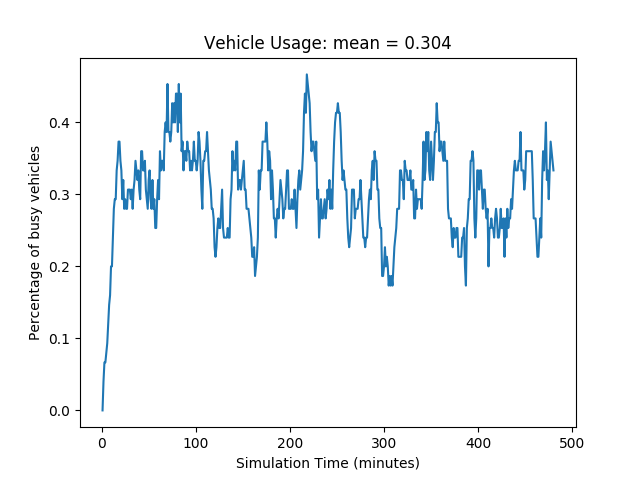
\includegraphics[width=0.75 \textwidth]{no_traffic_vehicles}

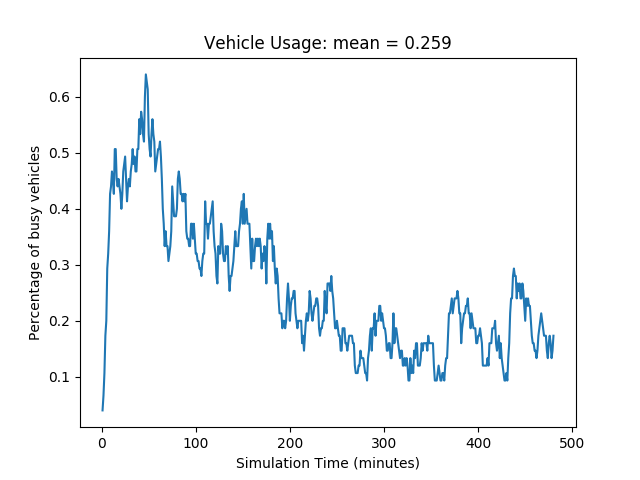
\includegraphics[width=0.75 \textwidth]{traffic_vehicles}

The reason we consider the vehicle usage over the number of pedestrians waiting to be picked up, is that the
customers are much noisier, but otherwise tell the same story. The additional noise likely comes from the
large number of customers that are picked up almost immediately. The plot below shows results for the same run
of the model as the traffic case above:

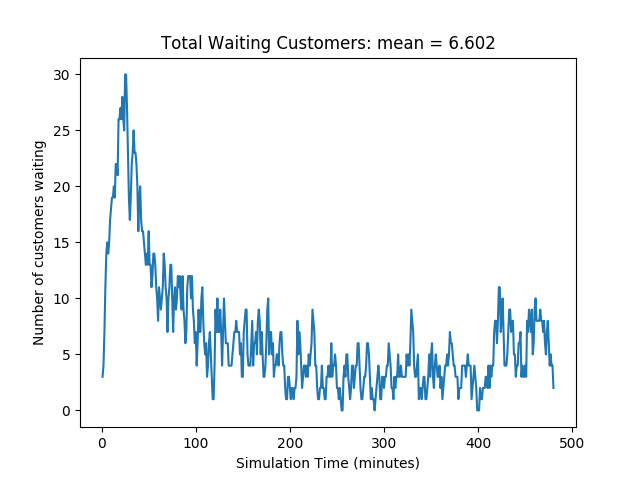
\includegraphics[width=0.75 \textwidth]{total_customers}

We also observe that our self-driving car model has better performance than the human driver model. We further see
that human drivers are superior to self-driving cars when the self driving cars are not subject to constant
rerouting:

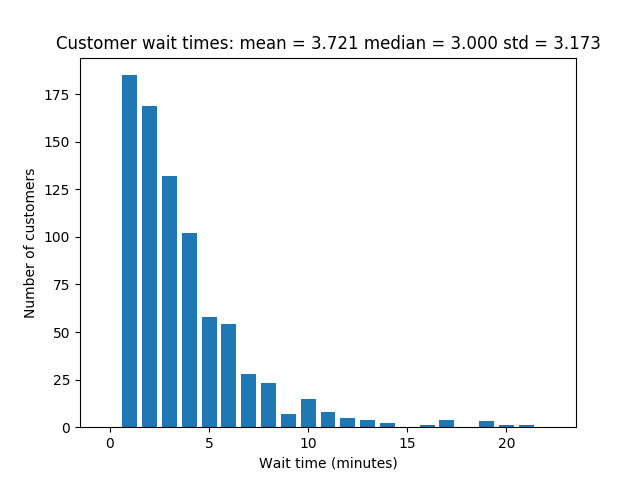
\includegraphics[width=0.75 \textwidth]{self_customers}

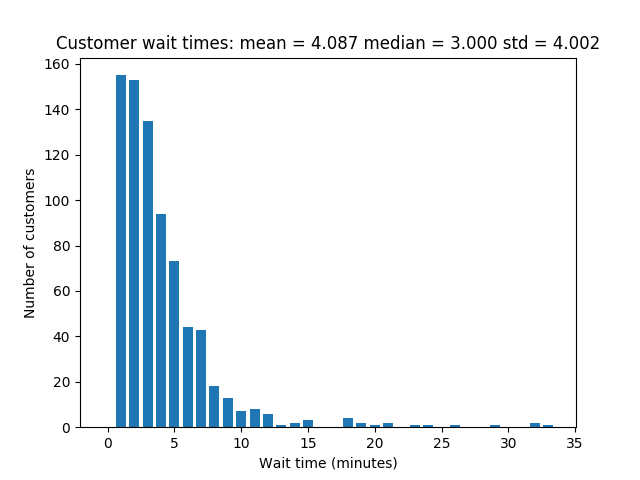
\includegraphics[width=0.75 \textwidth]{human_customers}

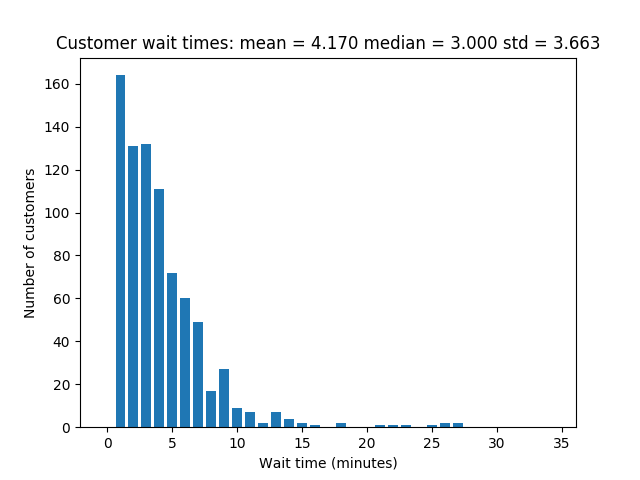
\includegraphics[width=0.75 \textwidth]{no_reroute_customers}

It was incorrectly stated in the presentation that the model was highly sensitive to the probability that humans
made errors. There was likely an error in labelling data, as the results could not be reproduced. The above plot
shows an initial error rate of 15\%, and the one below shows results for an error rate of 25\%. The results are
noticeably worse, but still better than without rerouting.

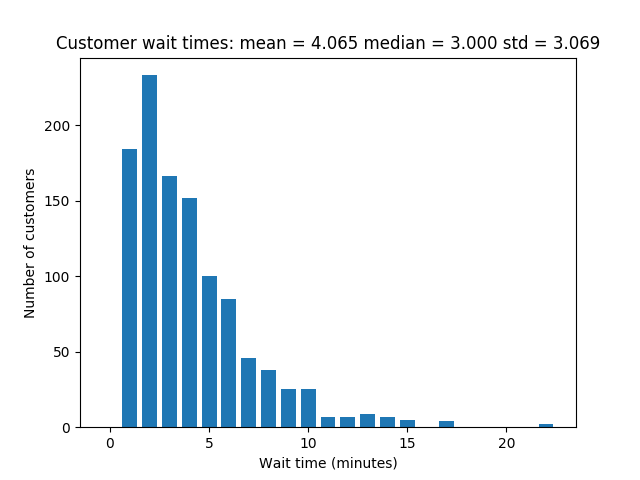
\includegraphics[width=0.75 \textwidth]{human_high_error_customers}

We found that in our cases with about 75 vehicles on 1210 intersections and 900 customers over the eight hours, that
around 450 total rerouting events occurred. That means that the number of times a vehicle received a route that was
different from its previous route was around 450. This helps explain the better results of the rerouting algorithm, as
that means there was on average around one reroute every single time step, as eight hours is 480 minutes, and each
step is a minute.

\section*{Conclusion}

Our model's robustness and our promising results leads us to think that our model is a good basis for further investigations into more realistic extension of our model. We believe the area in which our model could be extended would be on modelling the traffic in a more complex and realistic way. Our current model allows for cabs to move from node to node freely in any direction at a constant time. This is not an accurate model more a number of reasons. Firstly, the travel rate should depend on the traffic volume between intersections. Second, cars cannot usually just move back and forth in a city, and in a more realistic model, rerouting is sometimes simply not a possibility physically for the car, even if it is the most optimal path. An in-depth look at the traffic model would be a significant step forward for our model. The result in which human drivers with rerouting outperform self-driving cars without rerouting allows us to believe that this is a viable competitive model for current implementation before self-driving technology becomes too present among the transportation business.   

%
\pagebreak
%
%
% Now we start the appendices, with the new section name, "Appendix", and a
%  new counter, "I", "II", etc.
%
\appendix\label{section:feedback}

\section*{Feedback}

Here are a few questions and comments we would like to address about our model.\\

\textbf{Could you use the Manhattan distance even without all street intersections as nodes?} \\

Implementation of the Manhattan distance would be possible, but would prove to be more of a challenge to implement for ultimately a less accurate answer. The data that we've used stored the location of each intersection in latitude/longitude format and so it lends itself to be easily used using the Haversine function outlined in the paper. So in this case, the Haversine function is much more accurate and easier to implement than the Manhattan distance for curved surfaces. \\    

\textbf{Why do you care about the percentage of busy vehicles? How about the percentage of customers waiting?}\\

\textbf{What is the routing objective?} \\

The routing objective is minimize the overall distance of vehicle-customer pairs in a system. Our system changes in time and so we test whether updating this optimization calculation leads to significant reduced time over the whole simulation period.\\

\textbf{How do you decide that you have arrived at the destination if your cars move randomly?}\\

Our focus is to look on ways to reduce the wait time of customers. Consequently, the path and travel time after being picked up is not much of a concern. The customers are simply dropped off at some reasonable arbitrary time and location. \\


\textbf{What if there is an accident on one of the nodes, can the model capture that?}\\

No. This would be a good extension of our model and falls under the discussion of traffic in our model. See conclusion. \\

\textbf{What was the novel thing about your model?} \\

Re-routing, that is reassigning pairings of vehicles and customers, is not done by transportation firms and to our knowledge, is not analyzed in literature. See abstract, introduction.\\

\textbf{Is this an "Uber" model?} \\

The viability of our model to business would require more research. \\

\textbf{Did all intersections have the same peak time?}\\

Yes. This could be modified in the future. \\

\textbf{Is there an ideal distribution that you are trying to obtain for wait time?}\\

We expect our wait time to follow somewhat of a normal distribution, where most people will wait around the same amount of time, with ideally as few outliers as possible. We assumed that waiting for a cab for 30 mins would be rather rare, while wait for one for 5 mins would be more likely. This is what we see in our results, although due to little traffic simulation that our model has, the distribution is slightly skewed to lower wait times than we've expected. 

\appendix\label{section:contributions}

\section*{Contributions}

Richard Perryman was responsible for the analysis and implementation, both in writing and in code, of the path finding simulations as well as modeling the vehicle drivers. He was responsible to analyzing most the of the results. \\

Loic Nassif was responsible for the data analysis of the intersections, as well as the analysis and modeling of the city, both in writing and in code. He was also responsible for the background discussion. \\

Amjad Mobayed was responsible for the customer modelling section of our model. 

\appendix\label{section:references}
%
% Here's the first appendix, the list of references:
%
\bibliography{ascexmpl}
%
% And now for some pretty impressive notation.  In this example, I have used
%   the tabular environment to line up the columns in ASCE style.
%   Note that this and all appendices (except the references) start with
%   the \section command
%
%
\end{document}
